\documentclass[12pt]{article}
\usepackage[papersize={8.5in,11in}]{geometry}
\usepackage[pdftex]{graphicx}
\DeclareGraphicsExtensions{.pdf,.png,.jpg}
%
\usepackage{amsmath}
\usepackage{amsthm}
\usepackage{amssymb}
\usepackage{textcomp}
\usepackage[all]{xy}
\usepackage{fancyhdr}
\usepackage{hyperref}
\usepackage{verbatim}
\usepackage{algorithm}
\usepackage{algorithmic}
\usepackage{color}
\usepackage[usenames,dvipsnames,svgnames,table]{xcolor}
\usepackage{rotating}
\usepackage{wrapfig}
\usepackage{tikz}
\usetikzlibrary{shapes.geometric, arrows}
\usepackage{framed}
\usepackage[scaled=0.75]{FiraMono}
%\usepackage{newtxtt}

\usepackage{listings}
\lstset{language=python,frame=ltrb,framesep=5pt,basicstyle=\ttfamily,
 keywordstyle=\ttfamily\color{DarkRed}\bfseries,
%morecomment=[n][\textbf]{In\ [}{]\:},
%morecomment=[n][\textbf]{Out\ [}{]\:},
morecomment=[s][\color{blue}]{In\ [}{]\:},
morecomment=[s][\color{red}]{Out[}{]\:},
identifierstyle=\ttfamily\color{DarkBlue},
commentstyle=\color{OliveGreen},
stringstyle=\ttfamily\color{Orange},
showstringspaces=false,tabsize = 3}

\lstdefinelanguage{shell} {
commentstyle = \color{black},
keywordstyle = \color{black},
stringstyle = \color{black},
identifierstyle = \color{black},
morecomment=[s][\color{blue}]{In\ [}{]\:},
morecomment=[s][\color{red}]{Out[}{]\:},
 }


%
% this gives a little box for the end of a proof:
%
\def\endthrmbox{$\sqsubset \!\!\!\! \sqsupset$}

\newcommand{\dis}{\displaystyle}
 \def      \RR             {{\mathbb R}}
        \def      \NN             {{\Bbb N}}
        \def      \QQ             {{\Bbb Q}}
        \def      \CC             {{\Bbb C}}
        \def      \ZZ             {{\Bbb Z}}


        \def       \a              {{\alpha}}
        \def       \b              {{\beta}}
        \def       \d              {{\delta}}
        \def       \D              {{\Delta}}
        \def         \e              {{\varepsilon}}
        \def         \g              {{\gamma}}
        \def         \G              {{\Gamma}}
        \def       \l              {{\lambda}}
        \def       \L              {{\Lambda}}
        \def        \m               {{\mu}}
        \def         \n              {{\nabla}}
        \def       \var          {{\varphi}}
        \def         \s              {{\sigma}}
        \def       \Sig          {{\Sigma}}
        \def       \Om          {{\Omega}}

        \def       \t              {{\tau}}
        \def         \th             {{\theta}}
        \def       \O              {{\Omega}}
        \def       \o              {{\omega}}
        \def         \z              {{\zeta}}
       \def        \P             {{\Phi}}
       \def        \p             {{\phi}}
        %Other macros

        \def       \iy              {{\infty}}
        \def         \pa             {{\partial}}
        \def         \div           {{\rm div}}
         \def       \na            {{\nabla}}


%\renewcommand\baselinestretch{1.3}
%% The following block is for narrow margins:
\setlength{\topmargin}{-0.9in}
\setlength{\textheight}{9.50in}
\setlength{\oddsidemargin}{-0.375in}
\setlength{\evensidemargin}{-0.375in}
\setlength{\textwidth}{7.25in}
\setlength{\parindent}{0pt}
\setlength{\parskip}{2pt}
%% end page descript.




\usepackage[compact,explicit]{titlesec}
\titleformat{\section}[runin]{\large\bfseries}{}{0pt}{\titlerule[1.5pt]\newline\vspace*{-4pt}\quad
\newline}%[\vspace{0.01ex}{\titlerule[1.5pt]}]

\usepackage[final]{pdfpages}

\title{Homework \#2}
\author{Kyle MacMillan, \\Remington Bullis}


\begin{document}
\maketitle

Having now had a half-semester to digest and process information about nature-inspired computing approaches like simulated annealing and various implementations of evolutionary algorithms, Homework \#2 challenged us to tackle a nontrivial task: image reproduction. Our official bidding was to use an evolutionary algorithm (with our own quirks)  to evolve the closest approximation of a given image. Our implementation focused on a very robust generation-to-generation reproduction system using both crossover and point mutations. This approach yielded remarkable results. 
\\ \\
\textbf{Note: }The repository for this paper can be found \href{https://github.com/macattackftw/ncGA}{here}. 
The \verb|README.md| contains a gif of our solution in action and a full suite of test results can be seen in the \verb|results| folder. A selection of these results can also be seen in Appendix A. 

\section{} %%  This will generate a numbered problem header.

\subsection{Initial Approach and Encoding}
Before programming could begin we needed to know \textbf{1)} the language with which we would write our project, and \textbf{2)} the exact algorithm we were implementing. Python was the obvious choice for quickly iterating and testing. Algorithm development started at the discussion of how exactly we were going to generate images. After some back and forth we decided to build our image reconstructions purely in grayscale, and with layered circles. One "epoch" would be completed to generate an optimal circle. Each epoch would consist of its own population which was to be evolved over a set number of generations, with the most fit individual pulled and added to the reconstruction. While computationally intensive this one-at-a-time approach was expected to be robust and consistently convergent. 
\\
Encoding the properties of a circle into a genome was quite simple. We used \verb|numpy| to define a datatype that held the following information:
\begin{itemize}
\item The circle's center coordinates, $(x, y)$
\item The circle's radius, $r$
\item the circle's intensity, or alpha value, $i$
\end{itemize}

The actual definition of our genome can be seen below:
\begin{lstlisting}
self.center = np.dtype([('x', np.float32), ('y', np.float32)])
self.genome = np.dtype([('center',self.center), ('radius', np.float32), ('intensity', np.float32) ])
\end{lstlisting}


\subsection{Measuring Individual Fitness}
Given a circle to be placed on the stack of circles, how do we determine how "fit" this individual is relative to any other circle? This question plagued us for days. Unlike a simple mathematical function one can't just plug a circle into an image and get a numeric out indicating progress. The circle's fitness depends on not only the information confined to its bounds, but also how the circle fits into the larger context of the image. Our initial approaches to generating a fitness function proved fruitless; one simply filled the image as quickly as possible with white, and another would produce results only slightly better than random circle placement. 

We eventually determined that, given a circle, we should:
\begin{enumerate}
\item Determine the number of pixels occupied by the circle, $n$
\item Generate the circle in a mask
\item Add this mask to the current circle stack, constructing  a prospective next-circle stack
\item Determine the total difference between this prospective stack and the actual image to be reconstructed, $e$
\item Formulate a normalization factor, $p = n/(total pixel count)$
\item Return a final fitness $e - n*p$
\end{enumerate}

Our function definition is as follows:
\begin{lstlisting}
def Fitness(self, individual):
  cx, cy, r = individual['center']['x'], individual['center']['y'], individual['radius']
  Y, X = np.ogrid[-cy:self.height - cy, -cx:self.width - cx]
  mask = X**2 + Y**2 <= r**2                   # Calculate mask
  # Where the magic begins
  pixel_count = np.sum(mask, dtype=np.float32)
  circle = mask * individual['intensity']
  art = self.art + circle 						     # Gen prospective stack

  return np.sum(np.abs(self.image - art)) - pixel_count * self.pixel_modifier
\end{lstlisting}

This fitness function tracks how well the circle improved its local area relative to its size. Once we had it in place, the stars aligned and things converged!

\subsection{Evolving a New Circle}
Our process of generating and selecting a new circle is somewhat involved. Each final circle is the product of a full evolutionary run with its own population. We follow the standard \textit{initialize population}$\rightarrow$\textit{mutate/crossover}$\rightarrow$\textit{test population fitness}$\rightarrow$\textit{select survivors}$\rightarrow$
\textit{breed next generation} pipeline in this process but have added in some interesting quirks to both the mutation/corssover and selection steps. 

\subsubsection{Mutation and Crossover}
Our crossover implementation is as simple as it gets: take two individuals and calculate the average $x$ and $y$ center positions and the radii. The mutation process is also straightforward but takes into account how many generations have been evolved up to that point. For each attribute $y$ of the circle to mutate:
\begin{enumerate}
\item Generate a Gaussian random number $p$, $\bar{x} = 0, \sigma = s$
\item Determine a proportional shift $\tilde{y} = p*y$
\item Calculate the new, mutated value $y^{\prime} = y + \tilde{y}$
\item Set $y = y^{\prime}$ 
\end{enumerate}
The distribution deviation $\sigma$ changes depending on generation count. For the first three generations $\sigma = 0.3$, for generations in the first half after the first three $\sigma = 0.2$, and for the last half of the generations $\sigma = 0.1$. This has the effect of tapering off the randomness of mutation variations as generation count increases and, hopefully, the individuals home in on local maxima. Simulated annealing can work alongside GAs!

We also implemented another mutation strategy for a specific case to be discussed later. This takes in a circle and explicitly mutates each attribute in both an increasing \textit{and} decreasing direction.

\subsubsection{Selection and Generation}
The approach we've taken to population evolution is a bit more complicated than ranked selection and breeding. Given a population ranked by fitness we select a top proportion (the "royalty") and have them interbreed Hapsburg-style to generate a collection of new individuals equal in size to the input "royalty". These are crossed-over, mutated, and added to the new population. Then, (if population size > six) we take the most fit individual, who is also royalty, and mutate it using the special-case mutation described above to generate six new individuals. These are added to the new population. The remaining slots in the new population are filled with randomly-generated individuals. Combining random individual generation, elitist interbreeding, and several mutations of the most-fit individual into the next generation leads to a very robust population which captures the highlights of the previous population without stepping on new innovation.  

\subsection{Results}
The algorithm described in the above sections functioned stupendously well. In initial testing it became clear even with small circle counts that the algorithm was converging quickly to reconstructions that contained core structural information of the original images. Figure \ref{fig:darwin_0050} shows this early tendency towards low-frequency, high-gain information clearly. As circle counts increased high-frequency information started appearing, with massive circle counts almost identical to the original image. Over a dozen examples of high-count reconstructions can be found in Appendix A. 
\begin{figure}[H]
\centering
\noindent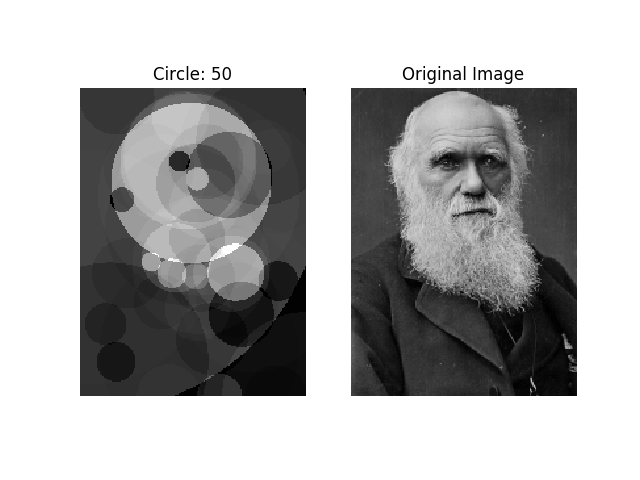
\includegraphics[width=0.4\textwidth]{../results/darwin/darwin_0050}
\noindent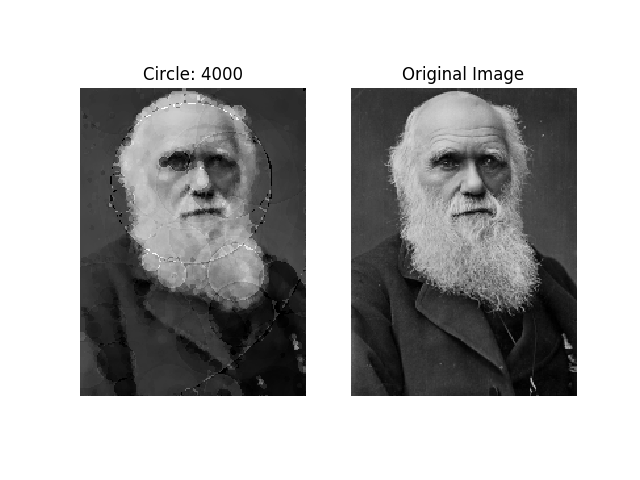
\includegraphics[width=0.4\textwidth]{../results/darwin/darwin_4000}
\caption{A portrait of Charles Darwin drawin with 50 and 4000 circles, repsectively. }
\label{fig:darwin_0050}
\end{figure}
There are some cases where the algorithm does not perform as well as expected. One case is that of cartoon characters: large swaths of empty space punctuated by very sharp, thin lines and hard gradients. Such information proved difficult for circles to represent using low circle counts. However, given a truly massive number of elements and time to work with, the algorithm did manage to reconstruct drawings satisfactorily. Figure \ref{fig:hobbes_0200} demonstrates this behavior well. 
\begin{figure}[H]
\centering
\noindent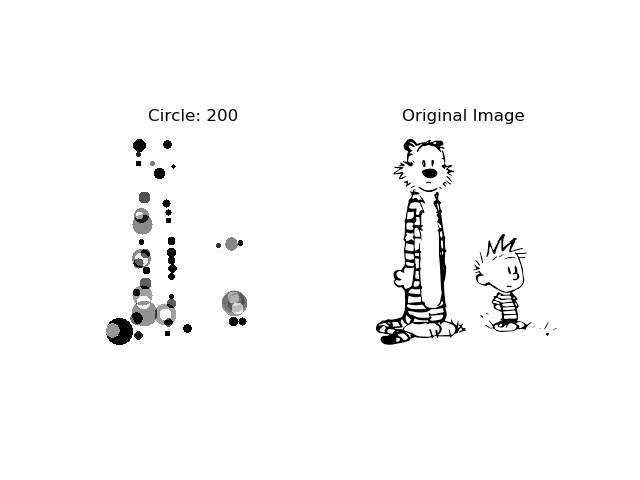
\includegraphics[width=0.4\textwidth]{../results/cartoons/hobbes_0200}
\noindent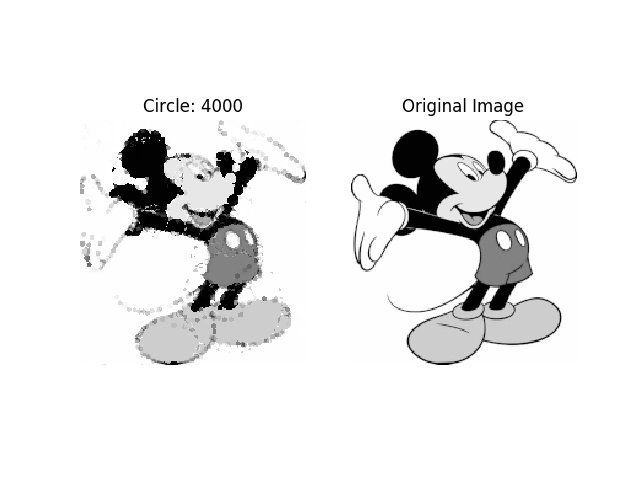
\includegraphics[width=0.4\textwidth]{../results/mickey/mickey_4000}
\caption{A portrait of Charles Darwin drawin with 50 and 4000 circles, repsectively. }
\label{fig:hobbes_0200}
\end{figure}
Curiously our initial expectations about larger populations leading to faster convergence were incorrect. 


\subsection{Conclusions}
Perhaps unsurprisingly, we discovered that robust genetic algorithms work well to (eventually) reproduce images from primitive shapes. While our implementation focused exclusively on recontruction of grayscale images with 

\begin{figure}[H]
\centering
\noindent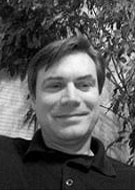
\includegraphics[width=0.65\textwidth]{../images/jmcgough}
\caption{The Persistence of Memory}
\label{fig:jmcgough}
\end{figure}

\begin{figure}[H]
\centering
\noindent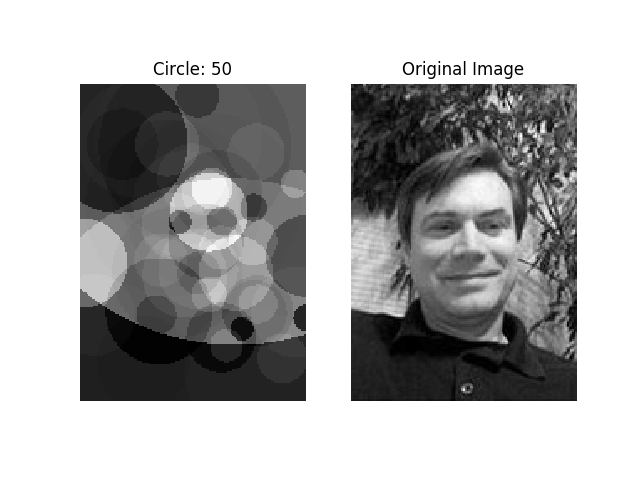
\includegraphics[width=0.65\textwidth]{../results/jmcgough/jmcgough_0050.png}
\caption{\textit{The Persistence of Memory} with 50 circles}
\label{fig:jmcgough_0050}
\end{figure}

\begin{figure}[H]
\centering
\noindent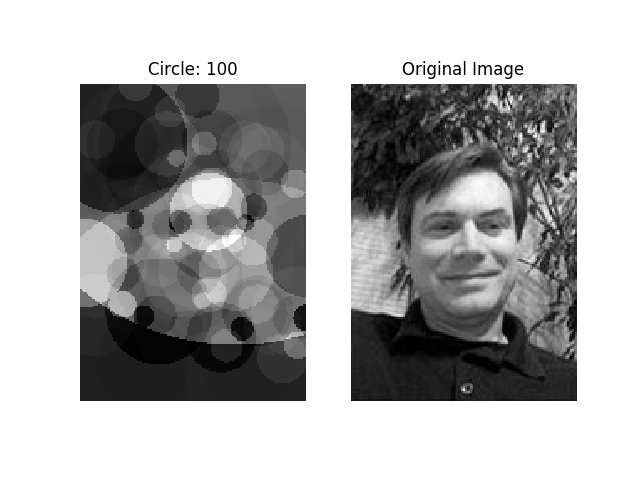
\includegraphics[width=0.65\textwidth]{../results/jmcgough/jmcgough_0100.png}
\caption{\textit{The Persistence of Memory} with 100 circles}
\label{fig:jmcgough_0100}
\end{figure}

\begin{figure}[H]
\centering
\noindent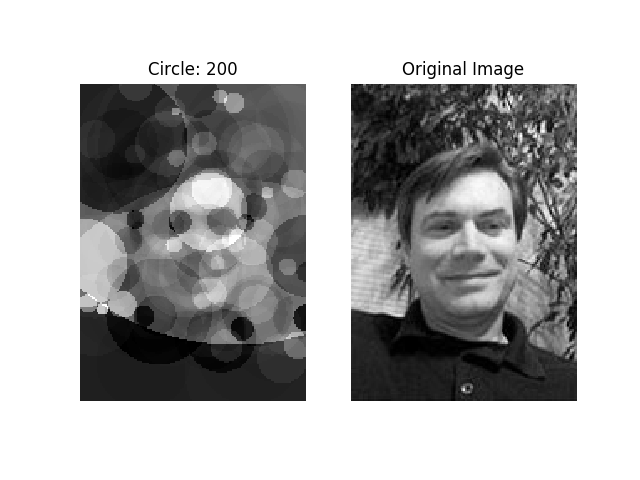
\includegraphics[width=0.65\textwidth]{../results/jmcgough/jmcgough_0200.png}
\caption{\textit{The Persistence of Memory} with 200 circles}
\label{fig:jmcgough_0200}
\end{figure}



\newpage
\subsection{Code}
\subsubsection{Best Circle}
\begin{lstlisting}
import numpy
\end{lstlisting}


\end{document}
